\section{Grafos}
Grafos são estruturas matemáticas que permitem codificar relacionamentos entre pares de objetos. As estruturas que podem ser representadas por grafos estão em toda parte e muitos problemas de interesse prático podem ser formulados como questões sobre certos grafos. Por exemplo, uma rota do metrô, e um labirinto.

Um grafo é composto por um conjunto de vértices e arestas conectando cada par de vértices com um relacionamento. Os vértices são os objetos da estrutura, que são representados por círculos, e as arestas são os relacionamentos existentes entre os vértices, sendo representadas por uma linha. Abaixo existem algumas figuras demonstrando a composição de um grafo.

\vspace{1cm}

\begin{figure}[!h]
    \centering
    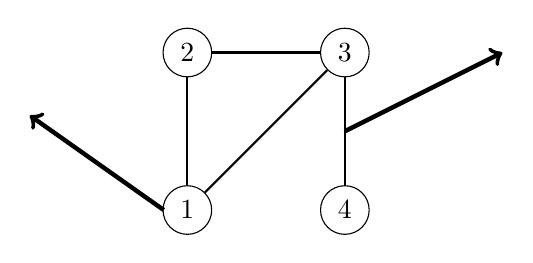
\begin{tikzpicture}
        \draw (0, 0) node[circle, black, draw](a1){1}
        (0, 2) node[circle, black, draw](a2){2}
        (2, 2) node[circle, black, draw](a3){3}
        (2, 0) node[circle, black, draw](a4){4};
        \draw[->, ultra thick] (2, 1) -- (4, 2);
        \draw[->, ultra thick] (-0.3, 0) -- (-2, 1.2);
        \draw[thick] (a1) -- (a2);
        \draw[thick] (a2) -- (a3);
        \draw[thick] (a3) -- (a4);
        \draw[thick] (a1) -- (a3);
    \end{tikzpicture}
    \caption{Exemplo de um grafo}    
\end{figure}

O grafo acima pode estar demonstrando o caminho de uma cidade para outra, sendo cada vértice uma cidade e as arestas as rodovias interligando cada cidade. As arestas presentes nesse grafo são: (1, 2), (1, 3), (2, 3), (3, 4).

\vspace{1cm}

\begin{figure}[!h]
    \centering
    \subfigure{
        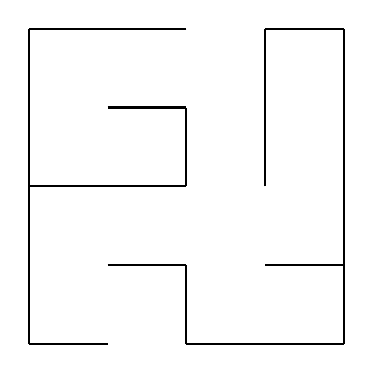
\begin{tikzpicture}
          \draw[thick] (0, 0) -- (1, 0);
          \draw[thick] (2, 0) -- (4, 0);
          \draw[thick] (4, 0) -- (4, 4);
          \draw[thick] (4, 4) -- (3, 4);
          \draw[thick] (2, 4) -- (0, 4);
          \draw[thick] (0, 4) -- (0, 0);
          
          %linhas horizontais
          \draw[thick] (1, 1) -- (2, 1);
          \draw[thick] (3, 1) -- (4, 1);
          \draw[thick] (0, 2) -- (2, 2);
          \draw[thick] (1, 3) -- (2, 3);
          
          %linhas verticais
          \draw[thick] (2, 0) -- (2, 1);
          \draw[thick] (2, 2) -- (2, 3);
          \draw[thick] (3, 2) -- (3, 4);
        \end{tikzpicture}
    }
    \quad
    \subfigure{
        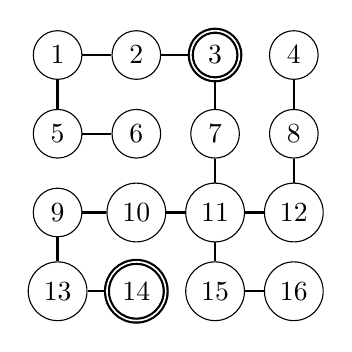
\begin{tikzpicture}
            %vértices
            \draw (1, 4) node[circle, black, draw](a13){13}
            (2, 4) node[circle, double, black, draw, thick](a14){14}
            (3, 4) node[circle, black, draw](a15){15}
            (4, 4) node[circle, black, draw](a16){16}
            (1, 5) node[circle, black, draw](a9){9}
            (2, 5) node[circle, black, draw](a10){10}
            (3, 5) node[circle, black, draw](a11){11}
            (4, 5) node[circle, black, draw](a12){12}
            (1, 6) node[circle, black, draw](a5){5}
            (2, 6) node[circle, black, draw](a6){6}
            (3, 6) node[circle, black, draw](a7){7}
            (4, 6) node[circle, black, draw](a8){8}
            (1, 7) node[circle, black, draw](a1){1}
            (2, 7) node[circle, black, draw](a2){2}
            (3, 7) node[circle, double, black, draw, thick](a3){3}
            (4, 7) node[circle, black, draw](a4){4};
            
            %arestas
            \draw[thick] (a1) -- (a2);
            \draw[thick] (a1) -- (a5);
            \draw[thick] (a2) -- (a3);
            \draw[thick] (a5) -- (a6);
            \draw[thick] (a3) -- (a7);
            \draw[thick] (a7) -- (a11);
            \draw[thick] (a4) -- (a8);
            \draw[thick] (a8) -- (a12);
            \draw[thick] (a9) -- (a10);
            \draw[thick] (a10) -- (a11);
            \draw[thick] (a11) -- (a12);
            \draw[thick] (a11) -- (a15);
            \draw[thick] (a9) -- (a13);
            \draw[thick] (a13) -- (a14);
            \draw[thick] (a15) -- (a16);
        \end{tikzpicture}
    }
    \caption{Representando um labirinto em um grafo}
\end{figure}

Podemos observar, através do grafo acima, que para sair do labirinto será necessário passar pelas arestas: (3, 7), (7, 11), (11, 10), (10, 9), (9, 13), (13, 14). 

\subsection{Conceitos Básicos de um Grafo}

\subsubsection{Grafos Direcionados}
Em um grafo direcionado as relações representadas pelas arestas possuem sentido definido. Isso significa que as arestas só podem ser seguidas em uma única direção. Em grafos direcionados, as arestas são pares ordenados de vértices, saindo de um, a origem, e indo para o outro, o destino.
\subsubsection{Grafos Não-Direcionados}
\subsubsection{Grafos Ponderados}

\subsection{Representação de um Grafo}
Uma questão importante é como representar um grafo no computador, para isso, existem dois tipos principais de representações, Matriz de Adjacência e Lista de Adjacência.

\subsubsection{Matriz de Adjacência}
\subsubsection{Lista de Adjacência}

\subsection{Busca em Largura}
\subsection{Busca em Profundidade}

\vspace{1cm}
\rule{\textwidth}{0.4pt}
\large{\textbf{Exercícios}}\\

\begin{itemize}
    \item \textbf{1076} - Desenhando Labirintos
    \item \textbf{1082} - Componentes Conexos
\end{itemize}

\newpage